\documentclass[17pt]{beamer}
\usepackage{graphicx}
\usepackage{tikz}
\usepackage{tikz-cd}
\usepackage{amsfonts}
\usepackage{amssymb}
\usepackage{amsmath}
\usepackage{amscd}
\usepackage{amsthm}
\usepackage{bbm}
\usepackage{fourier}
\usepackage[utf8]{inputenc}
\title{$2$-categories of theories}
\author{Hans Halvorson}
\date{July 2018}
\setbeamertemplate{footline}{}
\setbeamertemplate{page number in head/foot}[totalframenumber]
\setbeamertemplate{navigation symbols}{\footnotesize\usebeamertemplate{page number in head/foot}}
\setbeamercolor{normal text}{fg=black,bg=white}
\setbeamercolor{alerted text}{fg=red}
\setbeamercolor{example text}{fg=black}
\usepackage[absolute,overlay]{textpos}
\newcommand{\arrowtcupp}[2]{\arrow[bend left=50, ""{name=U, below,inner sep=1}]{#1}\arrow[Rightarrow,from=U,to=MU,"#2"]}
\newcommand{\arrowtclow}[2]{\arrow[bend right=50, ""{name=L,inner sep=1}]{#1}\arrow[Rightarrow,from=LM,to=L]{}[]{#2}} % if you want to change some parameter of the label.
\newcommand{\arrowtcmid}[2]{\arrow[""{name=MU,inner sep=1},""{name=LM,below,inner sep=1}]{#1}[pos=.1]{#2}}
\newcommand{\dummy}{\textcolor{white}{\bullet}}
\usepackage{adjustbox}
\usetikzlibrary{arrows}
\begin{document}
\def\2{\mathcal}
\def\7{\mathfrak}

\begin{frame}

\maketitle  

\end{frame}

\begin{frame}{The Objective}

  explicate relations between scientific theories

  \bigskip {\small e.g. \textit{equivalent} | \emph{reducible to} |
    \emph{simpler than} | } \newline {\small \emph{more ontologically
  parsimonious than} | } \newline  {\small \emph{imputes less structure than}}

\bigskip beyond spatial and financial metaphors

%% spatial: is part of, is contained in [compare with Kant on the
%% analytic], contain no more information [Feintzeig]

%% financial: more costly, more commitments, forced on us [Feingtzeig]

\end{frame}

\begin{frame}{\small $3$ paradoxes}

  \begin{itemize}
  \item reduction: if $B$ reducible to $A$, then $B$ says nothing more
    than $A$
  \item equivalence: if $A$ and $B$ are equivalent, then they are the same
  \item deduction: if $B$ is deducible from $A$, then $B$ says nothing more than $A$
  \end{itemize}  

\end{frame}  




\begin{frame}{\small $2$ old approaches}

 \begin{description}
 \item[syntactic] a theory is a set of sentences
 \item[semantic] a theory is a collection of models
  \end{description}

\end{frame}  

\begin{frame}{\small $2$ new approaches}

  \begin{description}
  \item[syntactic] theories are syntactic structures \newline
    $1$-cells are translations \newline
    $2$-cells are functional relations
  \item[semantic] theories are categories of models \newline $1$-cells are
    functors \newline $2$-cells are natural transformations
  \end{description}

\end{frame}

\begin{frame}[fragile]{\small categories, functors, natural
    transformations}


  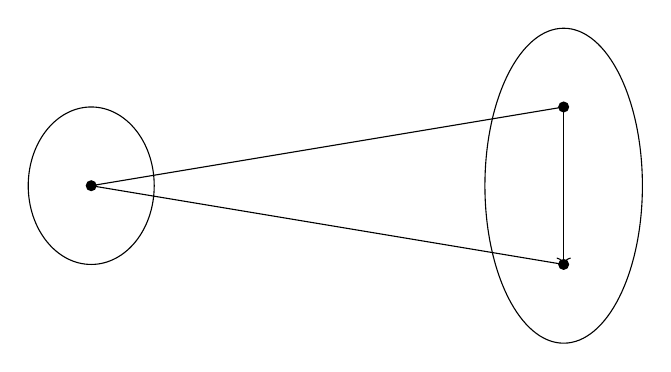
\begin{tikzpicture}
    \draw (0,0) ellipse (0.8cm and 1cm);
    \draw (6,0) ellipse  (1cm and 2cm);
    \path coordinate (a) at (0,0);
    \fill [black,opacity=1] (a) circle (2pt);
    \path coordinate (b) at (6,-1);
    \fill [black,opacity=1] (b) circle (2pt);
    \path coordinate (c) at (6,1);
    \fill [black,opacity=1] (c) circle (2pt);
    \draw (a)--(b) (a)--(c);
    \draw [->] (c)--(b);
\end{tikzpicture}


\end{frame}  




\begin{frame}[fragile]{\small $2$-categorical concepts}

%% examples of 2-categories: categories, 


\adjustbox{scale=1.2,center}{    
  \begin{tikzcd}[column sep=2cm]
A
\arrow[r, bend left=60, ""{name=q, below,}]
\arrow[r, bend left=0,""{name=k, above,}]
\arrow[r, ""{name=z, below,}]
  \arrow[r, bend right=60, ""{name=s, above,}] 
  \arrow[Rightarrow,from=q, to=k]
  \arrow[Rightarrow,from=z, to=s]
  & B
    \arrow[r, bend left=60, ""{name=a, below,}]
  \arrow[r, bend right=60,""{name=b, above,}] 
  \arrow[Rightarrow,from=a, to=b]
  & C 
\end{tikzcd} }

\bigskip

horizontal composition

vertical composition



\end{frame}

\begin{frame}[fragile]{\small exchange law}

\adjustbox{scale=0.9,center}{
\begin{tikzcd}[column sep=2cm]
    \dummy \arrowtcmid{r}{}
    \arrowtcupp{r}{\alpha}\arrowtclow{r}{\alpha\smash'} & \ast \arrowtcmid{r}{} \arrowtcupp{r}{\beta}\arrowtclow{r}{\beta\smash'} & \dummy
\end{tikzcd}
=
\begin{tikzcd}[column sep=2cm, row sep=-.15cm]
\dummy \arrowtcmid{r}{}\arrowtcupp{r}{\alpha} & \dummy \arrowtcmid{r}{}\arrowtcupp{r}{\beta} & \dummy \\
& \circ & \\
\dummy \arrowtcmid{r}{}\arrowtclow{r}{\alpha\smash'} & \dummy \arrowtcmid{r}{}\arrowtclow{r}{\beta\smash'} & \dummy
\end{tikzcd}
}

\[ (\beta '\circ \beta )\ast (\alpha '\circ \alpha ) \: = \: (\beta
  '\ast \alpha ')\circ (\beta \ast \alpha ) \]


\end{frame}

\begin{frame}{\small $2$-categorical concepts}

  %% refer here to Thomas on forgetting structure ?
  %% refer here to Feintzeig on reduction as adjunction ?

  \begin{itemize}
  \item full, faithful, essentially surjective  
  \item equivalence pair
  \item adjoint pair
  \item $2$-limits (e.g. comma category)
  \end{itemize}


\end{frame}


\begin{frame}{\small truisms about equivalence}

  \begin{itemize}
  \item geometry with points $\cong$ geometry with
    lines 
  \item every many-sorted theory $\cong$ some single-sorted
    theory
  \item category theory $\cong$ arrows-only category theory
  \end{itemize}




\end{frame}




\begin{frame}{\small truisms about reducibility}

\begin{itemize}
  \item $\mathbb{Q}$ is reducible to $\mathbb{Z}$
  \item $\mathbb{C}$ is reducible to $\mathbb{R}$
  \item geometry with points and lines is reducible to geometry with
    lines
  \end{itemize}

%% we want to understand in what sense talk about the rational numbers
%% can be translated into talk about the integers
  

\end{frame}


\begin{frame}{\small Extension by definition}

Defining new sort symbols

\bigskip
\begin{tabular}{l l}
product & $\sigma _1\times \sigma _2$ \\
coproduct & $\sigma _1+\sigma _2$ \\
subsort & $i:\sigma '\to \sigma$ \\
quotient & $e:\sigma\to\sigma '$ \end{tabular}

\end{frame}


\begin{frame}{\small Definitional (Morita) equivalence}

  $T_1$ and $T_2$ are \emph{Morita equivalent} just in case there are
  Morita extensions $T_1,T_1^1,\dots ,T_1^n$ and
  $T_2,T_2^1,\dots ,T_2^m$ such that $T_1^n$ and $T_2^m$ are logically
  equivalent.

  



\end{frame}



\begin{frame}{\small translation generalized}

  A \emph{reconstrual} $F:\Sigma\to\Sigma '$ assigns to each sort $\sigma\in\Sigma$:
  \begin{itemize}
    \item a finite sequence $F(\sigma
      )$ of sorts of $\Sigma '$
    \item a domain formula
      $D_\sigma$
    \item a relation $E_\sigma$ \end{itemize}

  


\end{frame}

\begin{frame}{\small 2-cells}

  A $2$-cell $\chi :F\Rightarrow G$ consists of a family $\chi
  _\sigma$ of $\Sigma '$-formulas such that each $\chi _\sigma$ is a
  $T'$-provably functional relation from $D^F_\sigma$ to $D^G_\sigma$.


\end{frame}



\begin{frame}[fragile]{\small Duality}

  \adjustbox{scale=1.2,center}{

  \begin{tikzcd}
    T \arrow{r}{F} & T' \\
    \mathrm{Mod}(T) & \mathrm{Mod}(T') \arrow{l}{F^*} \end{tikzcd} }

\end{frame}


\begin{frame}{\small Hudetz on reduction}

  \begin{enumerate}
  \item limiting case reductions
  \item theory embeddings
    \begin{enumerate}
    \item embedding of theorems (Nagel)
    \item embedding of models (Suppes)
    \end{enumerate}
  \end{enumerate}


\end{frame}









\begin{frame}{\small Washington's first theorem}

  Morita equivalent $\Longrightarrow$ intertranslatable

  \bigskip
  The reduction translation $R:T^+\to T$

  \vspace{2em}
  
  \begin{tabular}{l l | l l}
    $x=y$ & & & $x_1=y_1\wedge x_2=y_2$ \\ \hline
    $x=y$ & & & $(\phi (z)\wedge x_1=y_1)\vee (\neg \phi (z)\wedge x_2=y_2)$ \end{tabular}


\end{frame}


\begin{frame}{\small Washington's second theorem}

intertranslatable $\Longrightarrow$ Morita equivalent


\end{frame}


\begin{frame}{\small examples}

  \begin{itemize}
  \item point geometry and line geometry
  \item mereological universalism and mereological nihilism
  \item category theory and arrows-only category theory  
\end{itemize}

  
\end{frame}


\begin{frame}{\small a problem for semantic accounts}

  %% bad functors

  We lack an intrinsic (and useful) description of a reasonable 
 semantic 2-category

  \begin{description}
  \item[objects] categories of models \dots but which ones?
  \item[$1$-cells] functors \dots but which ones?
  \item[$2$-cells] natural transformations
    \end{description}

\end{frame}


\begin{frame}{\small open questions}
  
  Can we give intrinsic descriptions of relevant classes of functors
  between categories of models?

  \begin{description}
  \item[Makkai] preserves ultraproducts
  \item[Awodey] continuous  
  \item[Hudetz] constructible
  \end{description}



\end{frame}


% \begin{frame}[fragile]{\small symmetry and quotienting}


%   \begin{tikzcd}



    




%     \end{tikzcd}




% \end{frame}

\begin{frame}{\small open questions}

  \begin{itemize}
  \item How to explicate limiting relations between theories?
  \item Bad question: Is $T'$ reducible to $T$? 
  \item Better question: In what ways is $T'$ reducible to $T$?
\end{itemize}



\end{frame}  


\end{document}



%%% Local Variables:
%%% mode: latex
%%% TeX-master: t
%%% End:
